\documentclass[../analysisII_notes.tex]{subfiles}
\begin{document}
\section{Aula 26 - 23 de Junho, 2025}
\subsection{Motivações}
\begin{itemize}
	\item Funções Definidas Implicitamente por Projeções;
	\item Teorema da Função Implícita.
\end{itemize}
\subsection{Funções Definidas Implicitamente por Projeções}
Um exemplo clássico dessa situação e que ilustra bem o que ocorre no caso geral é fornecido pela equação da circunferência unitária no plano, ou seja,
\[
	x^{2} + y^{2} = 1.
\]
Ela define implicitamente quatro funções com domínio máximo: escrevendo
\begin{align*}
	 & U^{+}\coloneqq \{(x, y):\;y\geq 0\},\; U^{-}\coloneqq \{(x, y):\;y \leq 0\}          \\
	 & V^{+}\coloneqq \{(x, y):\;x \geq 0\}, \;\&\; V^{-} \coloneqq \{(x, y):\; x \leq 0\},
\end{align*}
vemos que um ponto \((x, y)\in U^{+}\) satisfaz a equação da circunferência se, e somente se,
\[
	y^{2} = 1-x^{2} \Longleftrightarrow y = \sqrt[]{1-x},
\]
ou seja, se, e somente se, y pode ser escrito como \(y = f(x)\) para
\[
	f(x) = \sqrt[]{1-x^{2}},\quad -1\leq x\leq 1.
\]
Analogamente, um ponto \((x, y)\in U^{-}\) satisfaz
\[
	x^{2} + y^{2} = 1 \Longleftrightarrow y = -\sqrt[]{1-x^{2}}.
\]
\begin{figure}[H]
	\begin{center}
		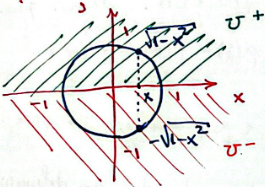
\includegraphics[height=0.5\textheight, width=0.5\textwidth, keepaspectratio]{./Images/circ_implicit_26.png}
	\end{center}
	\caption{funções implícitas a partir da equação da circunferência}
\end{figure}

\begin{def*}
	Seja \(f:U\subseteq \mathbb{R}^{m+n}\rightarrow \mathbb{R}\) uma função e p um ponto de U tal que \(f(p) = c.\) Dizemos que a equação \(f(x) = c\) \textbf{define implicitamente uma função numa vizinhança de p} quando existe uma vizinhança \(W\subseteq U\) de p tal que sua intersecção com a imagem inversa de c é o gráfico de uma função \(\xi :V\subseteq \mathbb{R}^{m}\rightarrow \mathbb{R}^{n}\), ou seja,
	\[
		W\cap f^{-1}(c) = \{(z, \xi (z)):\; z\in V\}. \square
	\]
\end{def*}
\begin{figure}[H]
	\begin{center}
		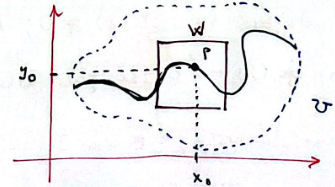
\includegraphics[height=0.5\textheight, width=0.5\textwidth, keepaspectratio]{./Images/implicit_function_26.png}
	\end{center}
\end{figure}

\begin{lemma*}
	Seja \(f:U\subseteq \mathbb{R}^{m}\rightarrow \mathbb{R}\) uma função tal que, para um ponto a de U e h um vetor de \(\mathbb{R}^{m}\) com \([a, a+h]\subseteq U\), tenhamos:
	\begin{itemize}
		\item[i)] A função f é contínua em \([a, a=h]\); e
		\item[ii)] Existe a derivada parcial de f na direção de h para todo x em \((a, a+h)\), ou seja,
		      \[
			      \exists\; \frac{\partial^{}f}{\partial h^{}}(x),\quad \forall x\in (a,a+h).
		      \]
	\end{itemize}
	Então, existe \(\theta \) em \((0, 1)\) tal que
	\[
		f(a+h) - f(a) = \frac{\partial^{}f}{\partial h^{}}(a+\theta h0.)
	\]
	Em particular, se f for diferenciável, então
	\[
		f(a+h) - f(a) = \sum\limits_{i=1}^{n}\frac{\partial^{}f}{\partial x_{i}^{}}(a+\theta h)\cdot h_{i},\; h = (h_1, \dotsc , h_{m}).
	\]
\end{lemma*}
\begin{proof*}
	Com efeito, escrevendo
	\begin{align*}
		\varphi : & [0, 1]\rightarrow \mathbb{R}           \\
		          & t\mapsto \varphi (t)\coloneqq f(a+th),
	\end{align*}
	vemos que \(\varphi \) está nas condições do teorema do valor médio e, consequentemente, existe um ponto \(\theta \) no intervalo \((0, 1)\) com
	\[
		\varphi (1) - \varphi (0) = \varphi '(\theta ).
	\]
	Calculando, então, \(\varphi '(\theta )\), chegamos em
	\[
		\varphi '(\theta ) = \lim_{t\to 0} \frac{\varphi (\theta +t) - \varphi(\theta )}{t} = \frac{\partial^{}f}{\partial h^{}}(a+\theta h),
	\]
	e a conclusão segue.

	O caso particular é um resultado da definição do diferencial:
	\[
		\frac{\partial^{}f}{\partial h^{}}(x) = f'(x)\cdot h = df(x)\cdot h = \left< \nabla f(x), h \right> = \sum\limits_{j=1}^{m}\frac{\partial^{}f}{\partial x_{j}^{}}(x)\cdot h_{j}.\; \text{\qedsymbol}
	\]
\end{proof*}
\hypertarget{implicit_function}{
	\begin{theorem*}[Teorema da Função Implícita]
		Seja \(f:U\subseteq \mathbb{R}^{m+1}\rightarrow \mathbb{R}\) uma função de classe \(\mathcal{C}^{1}\) e escrevamos os pontos de \(\mathbb{R}^{m+1}\) na forma \((x, y)\), sendo x um vetor em \(\mathbb{R}^{m}\) e y um número real. Seja, também, \(p=(x_{0}, y_{0})\) um ponto de U e escreva \(c=f(p).\) Nessas condições, se \(\frac{\partial^{}f}{\partial y^{}}(p)\) é deiferente de 0, então:
		\begin{itemize}
			\item[i)] Existem \(\delta \) e \(\varepsilon \), ambos positivos, tais que
			      \[
				      \overline{B}(x_{0}; \delta ) \times [y_{0}-\varepsilon , y_{0}+\varepsilon ] \subseteq U;\; \frac{\partial^{}f}{\partial y^{}}(x, y)\neq 0;
			      \]
			\item[ii)] Existe uma função \(\xi :B\rightarrow J\) de classe \(\mathcal{C}^{1}\) e tal que
			      \[
				      f^{-1}(c)\cap (B\times J) = \mathrm{Graf}(\xi );
			      \]
			\item[iii)] Para todo x em B,
			      \[
				      \frac{\partial^{}\xi }{\partial x_{i}^{}}(x) = -\frac{\frac{\partial^{}f}{\partial x_{i}^{}}(x, \xi (x))}{\frac{\partial^{}f}{\partial y^{}}(x, \xi (x))}.
			      \]
		\end{itemize}
	\end{theorem*}
}
\begin{proof*}
	(i) Suponhamos que \(\frac{\partial^{}f}{\partial y^{}}(p)\) é positivo. Da continuidade da função
	\[
		\frac{\partial^{}f}{\partial y^{}}:U\rightarrow \mathbb{R},
	\]
	obtemos \(\delta > 0 \) e \(\varepsilon  > 0\) como em (i). Logo,
	\[
		\frac{\partial^{}f}{\partial y^{}}(x, y)>0,\; \forall (x, y)\in B \times J.
	\]

	(ii) Com isso, notemos que, pela função que age por
	\[
		[y_{0}-\varepsilon , y_{0}-\varepsilon ]\ni y \mapsto f(x_{0}, y)\in \mathbb{R}
	\]
	ser crescente, temos
	\[
		f(x_{0}, y_{0}-\varepsilon ) < c < f(x_{0}, y_{0}+\varepsilon ),
	\]
	tal que podemos ir diminuindo \(\delta  > 0\) se necessário até fazer sentido impôr, para todo x em \(\overline{B}\), que
	\[
		f(x, y_{0}-\varepsilon ) < c < f(x, y_{0}+\varepsilon ),
	\]
	pois f é contínua. Desta maneira, fixado x em B, pela continuidade de
	\[
		J\ni y \mapsto f(x, y)\in \mathbb{R}
	\]
	e pelo Teorema do Valor Intermediário, existe \(\xi (x)\) em \(\overline{J}\) tal que
	\[
		f(x, \xi (x)) = c;
	\]
	necessariamente, então, \(\xi (x)\in J\), pois o mapa de y até f(x, y) é crescente. Além disso, \(\xi (x)\) é o único que satisfaz essa condição, provando o item (ii).

	iii) Para o cálculo das derivadas, fixados x em B e t não nulo, escrevamos
	\[
		h(t) = \xi (x+te_{i}) - \xi (x),
	\]
	tal que, para todo t diferente de 0,
	\[
		\xi (x + t e_{i}) = \xi (x) + h(t) \Rightarrow c = f(x+t e_{i}, \xi (x + t e_{i})) = f(x, \xi (x));
	\]
	ou, ainda,
	\[
		f(x+t e_{i}, \xi (x) + h(t)) = f(x, \xi (x)) = c.
	\]

	Pelo lema que provamos,
	\begin{align*}
		0 & = \sum\limits_{j=1}^{m}\frac{\partial^{}f}{\partial x_{j}^{}}((x, \xi (x)) + \theta \cdot (te_{i}, h(t)))\cdot h_{j} + \frac{\partial^{}f}{\partial y^{}}((x, \xi (x)), \theta (t e_{i}, h))\cdot h  \\
		  & \Longleftrightarrow \frac{\partial^{}f}{\partial x_{i}^{}}(x+\theta t e_{i}, \xi (x) + \theta h(t)) \cdot t + \frac{\partial^{}f}{\partial y^{}}(x+\theta t e_{i}, \xi (x) + \theta h(t))\cdot h(t).
	\end{align*}
	Como \(\xi \) é contínua (vide observação), \(h(t)\) tende a 0 conforme o próprio t tende, e podemos escrever
	\[
		\frac{\xi (x + te_{i})-\xi (x)}{t} = \frac{h(t)}{t} = - \frac{\frac{\partial^{}f}{\partial x_{i}^{}}(x+\theta t e_{i}, \xi (x) + \theta h(t))}{\frac{\partial^{}f}{\partial y^{}}(x + \theta te_{i}, \xi (x) + \theta h(t))} \rightarrow -\frac{\frac{\partial^{}f}{\partial x_{i}^{}}(x, \xi (x))}{\frac{\partial^{}f}{\partial y^{}}(x, \xi (x))}. \text{ \qedsymbol}
	\]
\end{proof*}
\begin{tcolorbox}[
		skin=enhanced,
		title=Observação,
		fonttitle=\bfseries,
		colframe=black,
		colbacktitle=cyan!75!white,
		colback=cyan!15,
		colbacklower=black,
		coltitle=black,
		drop fuzzy shadow,
		%drop large lifted shadow
	]
	A continuidade de \(\xi \) pode ser demostrada fixando x em B e uma sequência \(\{x_{\ell}\} \) em B também com \(x_{\ell}\) convergindo para x. Por definição,
	\[
		c = f(x_{\ell}, \xi (x_{\ell})),\; \forall \ell \in \mathbb{N}.
	\]
	Como \(\xi (x_{\ell})\in \overline{J}\), podemos supor que
	\[
		\xi (x_{\ell})\overbracket[0pt]{\longrightarrow}^{\ell \to \infty}y
	\]
	e, da continuidade de f, devemos ter
	\[
		c = f(x, y) \Rightarrow y = \xi (x).
	\]

	De fato, se fosse falso que \(\xi (x_{\ell})\rightarrow \xi (x)\), então existiria uma subsequência \(\{x_{\ell }' \}\) de \(\{x_{\ell}\}\) com, para um certo \(\alpha \),
	\[
		|\xi (x_{\ell}) - \xi (x)|\geq \alpha > 0,\; \forall \ell \in \mathbb{N}.
	\]
	Assim, repetindo o processo anterior, obteríamos outra subsequência \(\{x_{\ell }''\}\) tal que
	\[
		\xi (x_{\ell }'')\rightarrow \xi (x),
	\]
	contradizendo a desigualdade acima.
\end{tcolorbox}
\end{document}
